\mnDifficult
\begin{slikaDesno}{fig/wien.pdf}
    \PID 
    У колу са слике познати су параметри $R$ и $C$, а употребљен је идеалан напонски појачавач чије је 
    напонско појачање $A$. Побуда система је струје $i_{\rm G} = i_{\rm G}(t)$, а одзив је 
    излазни напон $v_{\rm I} = v_{\rm I}(t)$.
    \begin{enumerate}[label = (\alph*)]
        \item Одрети фунцкију преноса система $H(s) = \dfrac{V_{\rm I}(s)}{I_{\rm G}(s)}$. 
    \end{enumerate}
\end{slikaDesno}
\begin{enumerate}[label=(\alph*)]\refstepcounter{enumi}
    \item У зависности од параметра $A$, скицирати полове система $H(s)$ у комплексној равни. 
\end{enumerate}
\textit{Напомена:} Идеалан напонски 
појачавач подразумева да је улазна отпорност бесконачна, а излазна отпорност нулта. Односно, представља 
идеалан напоном контролисан напонски генератор.

\RESENJE

(а) Функција преноса се може одредити писањем једине једначине по методу потенцијала чворова за улазни чвор напонског
појачавача чији је напон $V_{\rm I}/A$, у облику 
\begin{equation}
    \dfrac{V_{\rm I}(s)}{A}
    \left(
        \dfrac{1}{R + \dfrac{1}{sC}}
        + 
        \dfrac{1}{R}
        +
        sC
    \right)
    = 
    I_{\rm G}(s)
    + 
    \dfrac{V_{\rm I}(s)}{R + \dfrac{1}{sC}}.
\end{equation}
%
\begin{figure}[b!]
    \centering
    \begin{subfigure}[t]{0.32\textwidth}
        \centering
        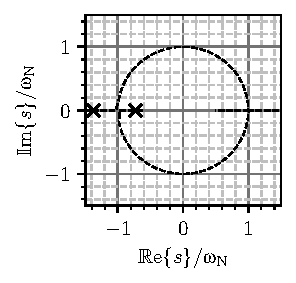
\includegraphics{fig/Q_polovi_1.pdf}
        \caption{$0 < Q < \dfrac{1}{2}$, $-\infty < A < 1$  }
    \end{subfigure}
    %
    \begin{subfigure}[t]{0.32\textwidth}
        \centering
        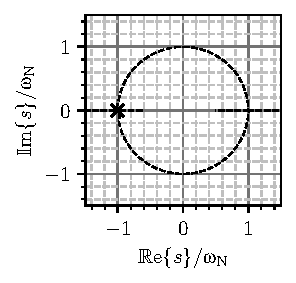
\includegraphics{fig/Q_polovi_2.pdf}
        \caption{$Q = \dfrac{1}{2}$, $ A = 1$}
    \end{subfigure}
    %
    \begin{subfigure}[t]{0.32\textwidth}
        \centering
        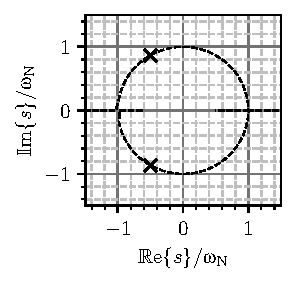
\includegraphics{fig/Q_polovi_3.pdf}
        \caption{$\dfrac{1}{2} < Q < \infty$, $1 < A < 3$}
    \end{subfigure}
    
    \begin{subfigure}[t]{0.32\textwidth}
        \centering
        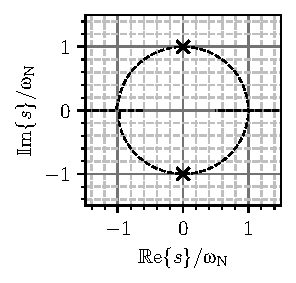
\includegraphics{fig/Q_polovi_4.pdf}
        \caption{$|Q| \to \infty$, $ A = 3$}
    \end{subfigure}
    %
    \begin{subfigure}[t]{0.32\textwidth}
        \centering
        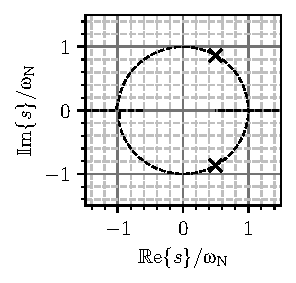
\includegraphics{fig/Q_polovi_5.pdf}
        \caption{$-\infty < Q < -\dfrac{1}{2}$, $3 < A < 5$}
    \end{subfigure}
    %
    \begin{subfigure}[t]{0.32\textwidth}
        \centering
        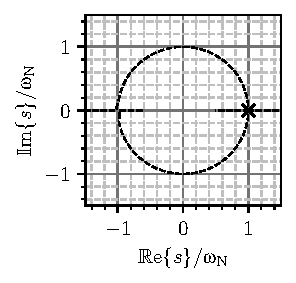
\includegraphics{fig/Q_polovi_6.pdf}
        \caption{$Q = -\dfrac{1}{2}$, $A = 5$}
    \end{subfigure}
    \caption{Положај полова у зависности од $Q$-фактора. Са променом $Q$-фактора, полови се крећу по испрекиданој области.}
    \label{fig:\ID.polovi}
\end{figure}
%
Решавањем дате једначине по излазном напону и даљим сређивањем налази се 
\begin{equation}
    H(s) = \dfrac{V_I(\rm s)}{I_{\rm G}(s)} = 
    \dfrac{AR(sRC + 1)}{ s^2(RC)^2 + (3-A)RCs + 1 }
\end{equation}
Заменом природне кружне учестаности за $RC$ коло $\upomega_{\rm N} = \dfrac{1}{RC}$, добијени израз се може 
записати као 
\begin{equation}
    H(s) = AR \dfrac{ \dfrac{s}{\upomega_{\rm N}} + 1}{ \dfrac{s^2}{\upomega_{\rm N}^2} + \dfrac{3 - A}{\upomega_{\rm N}}s + 1  }
    = AR 
    \dfrac{\upomega_{\rm N} s }{s^2 + \dfrac{\upomega_{\rm N}}{\frac{1}{3-A} }s + \upomega_{\rm N}^2  }.
\end{equation}
У добијеном изразу уочавамо облик имениоца који представља пар полова чији је $Q$-фактор дат као $Q = \dfrac{1}{3-A}$, па се на основу тога 
може дискутовати понашање овог система. У случају када је $Q < \dfrac{1}{2}$, односно $A < 1$, тада су полови реални, док су у супротном
случају $A > 1$ они пар комплексно конјугованих полова. У изузетном случају када је $A = 1$ постоји један двоструки реални пол. 
Различите конфигурације полова система илустроване су на слици \ref{fig:\ID.polovi}. Нагласимо да се $Q$-фактор у литератури
не дефинише за нестабилне системе, што се овде одразило на случајеве када су полови у десној комплексној полуравни. 

У овом случају, слично као у задатку \ref{zad:klatno}, приметно је кретање полова приликом промене једног од параметара
система. Познвавање ове појаве омогућује добар увид у механизам стабилности система. Када су полови система на имагинарној
оси, односно када је $A = 3$, тада је сам систем маргинално стабилан. На пример, такво коло се може користи као принципска
основа за пројектовање осцилатора. Коло илустровано у овом задатку је конкретан пример 
\textit{Осцилатора са Виновим мостом} (енг. \textit{Wien Bridge Oscillator}).

